% ****** Start of file apssamp.tex ******
%
%   This file is part of the APS files in the REVTeX 4.1 distribution.
%   Version 4.1r of REVTeX, August 2010
%
%   Copyright (c) 2009, 2010 The American Physical Society.
%
%   See the REVTeX 4 README file for restrictions and more information.
%
% TeX'ing this file requires that you have AMS-LaTeX 2.0 installed
% as well as the rest of the prerequisites for REVTeX 4.1
%
% See the REVTeX 4 README file
% It also requires running BibTeX. The commands are as follows:
%
%  1)  latex apssamp.tex
%  2)  bibtex apssamp
%  3)  latex apssamp.tex
%  4)  latex apssamp.tex
%
\documentclass[%
 reprint,
%superscriptaddress,
%groupedaddress,
%unsortedaddress,
%runinaddress,
%frontmatterverbose, 
%preprint,
%showpacs,preprintnumbers,
%nofootinbib,
%nobibnotes,
%bibnotes,
 amsmath,amssymb,
 aps,
%pra,
%prb,
%rmp,
%prstab,
%prstper,
%floatfix,
]{revtex4-1}

\usepackage{graphicx}% Include figure files
\usepackage{dcolumn}% Align table columns on decimal point
\usepackage{bm}% bold math
%\usepackage{hyperref}% add hypertext capabilities
%\usepackage[mathlines]{lineno}% Enable numbering of text and display math
%\linenumbers\relax % Commence numbering lines

%\usepackage[showframe,%Uncomment any one of the following lines to test 
%%scale=0.7, marginratio={1:1, 2:3}, ignoreall,% default settings
%%text={7in,10in},centering,
%%margin=1.5in,
%%total={6.5in,8.75in}, top=1.2in, left=0.9in, includefoot,
%%height=10in,a5paper,hmargin={3cm,0.8in},
%]{geometry}
% Using Blindtext
\usepackage{blindtext}
%Math-Environment
\usepackage{amsmath}
\usepackage{amssymb}
%Because Physics is cool
\usepackage{physics}
%Better SI-Units
\usepackage{siunitx}
%Use subfigs
\usepackage{subfig}
%Textcolors
\usepackage{color}
\usepackage{booktabs}
\DeclareSIUnit\century{century}
\DeclareSIUnit\year{yr}
\sisetup{
	per-mode=fraction,
	%	fraction-function=\tfrac
}

% New/Renewing Commands
\newcommand{\eV}{\electronvolt}
\newcommand{\keV}{\kilo\electronvolt}
\newcommand{\meV}{\mega\electronvolt}
\newcommand{\gray}{\rowcolor[gray]{.90}}
\newcommand{\degr}{^{\circ}}
\newcommand{\tit}[1]{\textit{#1}}
\newcommand{\baf}{BaF$_2$}
\newcommand{\pwo}{PbWO$_4$}
\newcommand{\ten}[1]{$10^{#1}$}
\newcommand{\orb}[2]{$#1^{#2}$}
\newcommand{\stat}[2]{$#1_{#2}$}
\newcommand{\ft}[2]{$#1\rightarrow#2$}
\newcommand{\sr}{$^{90}$Sr}
\newcommand{\co}{$^{60}$Co}
\newcommand{\eu}{$^{152}$Eu}
\newcommand{\cs}{$^{137}$Cs}
\newcommand{\ba}{$^{133}$Ba}
\newcommand{\na}{$^{22}$Na}
\newcommand{\ka}{$^{40}$Ka}

\begin{document}

%\preprint{APS/123-QED}

\title{Development of a SiPM-based readout-module for the characterization of various scintillator materials}% Force line breaks with \\
%\thanks{A footnote to the article title}%

\author{Lukas Nies}
\email{Lukas.Nies@physik.uni-giessen.de}
%\altaffiliation[Also at ]{Physics Department, XYZ University.}%Lines break automatically or can be forced with \\
\author{Hans-Georg Zaunick}%
\author{Kai-Thomas Brinkmann}
% \email{Second.Author@institution.edu}
\affiliation{%
 II. Institute of Physics, University of Giessen\\
 %This line break forced with \textbackslash\textbackslash
}%

%\collaboration{MUSO Collaboration}%\noaffiliation

%\author{Charlie Author}
% \homepage{http://www.Second.institution.edu/~Charlie.Author}
%\affiliation{
% Second institution and/or address\\
% This line break forced% with \\
%}%
%\affiliation{
% Third institution, the second for Charlie Author
%}%
%\author{Delta Author}
%\affiliation{%
% Authors' institution and/or address\\
% This line break forced with \textbackslash\textbackslash
%}%

%\collaboration{CLEO Collaboration}%\noaffiliation

\date{\today}% It is always \today, today,
             %  but any date may be explicitly specified

\begin{abstract}

In this paper we discuss a general approach to use SiPMs in different electrical configurations in combination with numerous scintillator materials for applications in nuclear instrumentation, like calorimetry and timing. The "hybrid" configuration used in the PANDA detector was found to show fastest timing properties with several hundred $\si{\pico\second}$ response by combining the advantages of a large active area while avoiding high operation voltages and dark noise. A "parallel" configuration shows the largest light collection efficiency and is therefore suitable for energy measurements. Several calibration spectra were taken to measure the energy deposit of minimal ionizing cosmic muons in a $2\si{\centi\meter}$ thick \pwo{} crystal. \textcolor{red}{WORK IN PROGRESS} 
 
%An article usually includes an abstract, a concise summary of the work
%covered at length in the main body of the article. 
%\begin{description}
%\item[Usage]
%Secondary publications and information retrieval purposes.
%\item[PACS numbers]
%May be entered using the \verb+\pacs{#1}+ command.
%\item[Structure]
%You may use the \texttt{description} environment to structure your abstract;
%use the optional argument of the \verb+\item+ command to give the category of each %item. 
%\end{description}
\end{abstract}

%\pacs{Valid PACS appear here}% PACS, the Physics and Astronomy
                             % Classification Scheme.
%\keywords{Suggested keywords}%Use showkeys class option if keyword
                              %display desired
\maketitle

%\tableofcontents

%\section{\label{sec:level1}First-level heading}

Modern photodetector applications encounter a large spectrum of different experimental environments. Prerequisites, e.g. working within strong magnetic fields, providing large intrinsic amplification, independence on high operation voltage, and space restrictions lead to the development of a new type of detectors, the semiconductor diodes. The \tit{Silicon Photomultiplier} (SiPM) integrates a large number of \tit{avalanche photodiodes} as microcells within a small space. With a large intrinsic amplification of up to $10^6$, the SiPM comes in many different packaging sizes and works mainly with low voltage between $\SI{25}{\volt}$ and $\SI{85}{\volt}$. Its insensitivity to magnetic fields and single photon counting capability in combination with suited scintillators make SiPMs a valuable choice for modern challenging applications, i.e. \tit{nuclear magnetic resonance imaging}, \tit{positron emission tomography}, and high energy calorimetry and tracking. \\ \indent
The development of the scintillation tile hodoscope \cite{SciTil}, short SciTil, for the \tit{PANDA} detector at the future Facility for Antiproton and Ion Research (\tit{FAIR}) at the GSI Helmholtz Centre for Heavy Ion Research in Germany \cite{FAIR} necessitated the development of a small-scale photo readout system insensitive to the magnetic field of the detector. The Wien group chose SiPMs due to previously mentioned properties. Coupling multiple SiPMs in an array increases the effective active area and, thus, enhances the photon detection efficiency. \\ \indent
\begin{figure}[b!]
	%\centering
	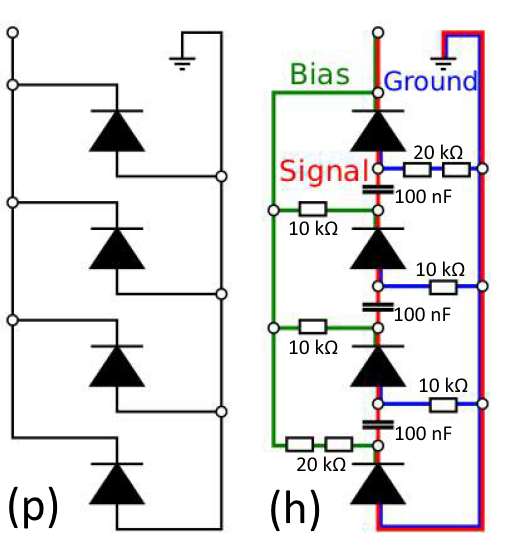
\includegraphics[width=0.5\linewidth]{./graphics/ch4/circuits.PNG}
	\caption{ Schematic of the two different SiPM configurations \cite{sebastian}. On the left is the ``parallel" configuration, on the right is the ``hybrid" configuration. The signal path is depicted in red, the bias current in green, and the ground in blue.  }
	\label{fig:PCB}
\end{figure}
In order to develop a general purpose SiPM array we designed in first iteration a printed circuit board (\tit{PCB}) which is able to host either a "parallel" or "hybrid" configuration by just adding or removing some resistors and capacities on the back of the board (see figure \ref{fig:PCB}). The signal is read out via a "bias-T" consisting of a resistor and a capacity which decouple the signal from the DC biasing.  \\ \indent
Attached to a plastic scintillator, comparing the raw and normalized signal shapes of a single SiPM with an array of four diodes in either parallel or hybrid configuration shows the fundamental differences of the methods. The signal amplitude for the hybrid configuration is roughly $\frac{1}{\sqrt{N}}$ compared to the amplitude of a single SiPM, where $N$ stands for the number of SiPMs per array. Driving the SiPM in parallel mode does not affect the signal amplitude. With a few nanoseconds the hybrid configuration has a considerably faster rising edge in respect to the parallel configuration where the latter tends to get slower as the number of SiPMs per array increases. Hence, SiPM-arrays in hybrid configuration are more suitable for time measurements whereas the parallel configuration is useful for energy measurements. \\ \indent
In order to yield breakdown and operation voltages, the temperature dependent current-voltage characteristics were studied. For this, the different configurations were wrapped with opaque tape to prevent occurrence of photon induced currents and put in a programmable refrigerator. For different temperatures between $-25^{\circ}C $ and $25^{\circ}C$ the SiPM-boards were biased and the IV-curves were measured with a custom made high voltage distribution board designed for operating the avalanche photo diodes of the electromagnetic calorimeter barrel of the PANDA detector \cite{chris}. \\ \indent
If a photo diode is driven in reversed bias mode the depletion layer between the p- and n-junction broadens and the built-in potential intensifies. At the breakdown voltage $U_{BD}$ electrons gain sufficient energy to create a self-sustained avalanche which leads to an exponential increase in current flowing. The breakdown voltages was determined by the intersection of a first order polynomial fit for the voltage area before breakdown and a second order polynomial for the region right after breakdown. \\ \indent
In order to find the optimal operation voltage $U_{OP}$, which is usually a few volts beyond breakdown, the minimum of the relative slope $\frac{dI}{dV}\frac{1}{I(V)}$ of the IV-curve was fitted. \\ \indent 
After scanning the IV-characteristics at different temperatures, the resulting breakdown temperature coefficient $k_{BD}$ for a single SiPM was in good agreement with the specifications of the manufacturer \cite{SiPM_Manual} (see \ref{tab:IV_cata}). The value for multiple SiPM does not seem to change (within the error). The coefficient for the operation voltage seems to add as the number of SiPMs increases: the four-SiPM array has a roughly four times higher values as the single SiPM. \\ \indent
\begin{table}[t!]
	\centering
	\begin{tabular}{ c|cc|cc } \toprule[2pt]
		& \multicolumn{2}{c|}{(s)-configuration} & \multicolumn{2}{c}{(h)- and (p)-configuration} \\
		T [$\si{\degreeCelsius}]$ & $V_{OP}$ [$\si{\volt}$] & $V_{BD}$ [$\si{\volt}$] & $V_{OP}$ [$\si{\volt}$] & $V_{BD}$ [$\si{\volt}$]  \\ \midrule
		-25 & $30.78\pm 3.99$ & $24.62\pm 2.89$ & $30.72\pm 0.47$ & $24.40\pm 3.67$ \\
		0 & $30.67\pm 0.42$ & $25.50\pm 0.60$ & $30.89\pm 0.15$ & $24.78\pm 0.03$ \\
		5 & $30.72\pm 0.32$ & $24.93\pm 0.15$ & $31.01\pm 0.59$ & $24.87\pm 0.04$ \\
		10 & $30.70\pm 0.35$ & $25.11\pm 0.44$ & $31.20\pm 0.32$ & $25.04\pm 0.04$ \\
		15 & $30.74\pm 0.28$ & $25.30\pm 0.14$ & $31.32\pm 0.68$ & $25.08\pm 0.01$ \\
		20 & $30.80\pm 0.23$ & $25.35\pm 0.05$ & $31.57\pm 0.75$ & $25.18\pm 0.03$ \\
		25 & $30.87\pm 0.45$ & $25.51\pm 0.23$ & $31.04\pm 2.11$ & $25.20\pm 0.06$ \\
		\midrule
		& $k_{OP}$ [$\si{\milli\volt\per\kelvin}$] & $k_{BD}$ [$\si{\milli\volt\per\kelvin}$] & $k_{OP}$ [$\si{\milli\volt\per\kelvin}$] & $k_{BD}$ [$\si{\milli\volt\per\kelvin}$]  \\
		& $6.79\pm 1.34$ & $23.66\pm 5.10$ & $23.67\pm 2.90$ & $19.30\pm 1.51$ \\
		\bottomrule[2pt]
	\end{tabular}
	\caption[Fit results for operation and breakdown voltages]{Fit results for operation and breakdown voltages. Since the same SiPMs were used for (h)- and (p)-configuration the results are the similar.}
	\label{tab:IV_cata}
\end{table}  
Since the diode is driven some volts beyond breakdown a probability is given that an avalanche is triggered by high energetic seed electrons. Because a SiPM is made up of thousands of microcells it is very likely to have plenty breakdowns in parallel every second. This effect can be suppressed by cooling where the high energetic part of the Boltzmann distributed electrons in the depletion layer gets shifted to lower thermal energies. \\ \indent
\begin{figure}[b!]
	\centering
	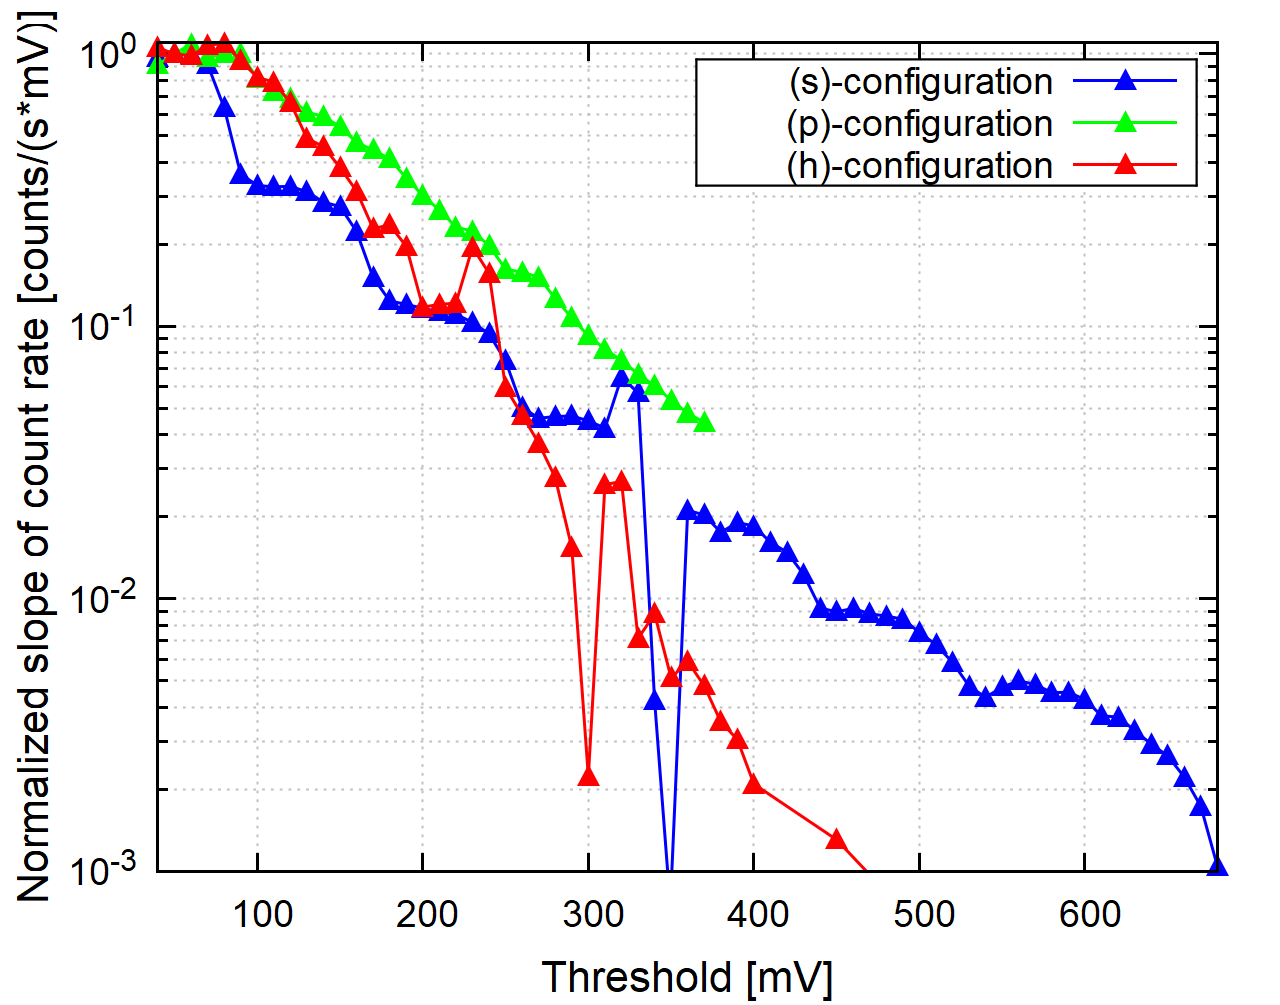
\includegraphics[width=0.9\linewidth]{./plots/dark_electron_spectrum/slope_countrate.png}
	\caption{Normalized slope of the dark count rate. The distinct step-like behavior for a single SiPM (blue) is clearly visible, while this subtle effect vanishes for multiple SiPMs (hybrid in red, parallel in green). Note the logarithmic scale. }
	\label{fig:dark_count_rate}
\end{figure} 
Examining this so-called dark count rate (signal without seeing a photon) of SiPMs is crucial for light sensitive applications. It is not recommended using SiPMs at room temperature for single photon counting since the dark count rate is high. By deploying different diode configurations in an opaque box and measuring the pulse height spectrum behind a pre-amplifier with an oscillator in persistence mode we investigated the dependence of count rate and threshold. For better visibility of this effect, the normalized dark count rate for different configurations is depicted in figure \ref{fig:dark_count_rate}. Because every microcell, if firing, contributes the same signal to the overall signal a single SiPM shows a step-like behavior for increasing thresholds. The possibility of three cells firing at the same time is suppressed by a factor of ten, and for six cells the suppression is almost a factor of hundred. In our setup, this effect can not be seen for multiple SiPMs. Every diode is biased by the same voltage but each SiPM has slightly different gain, therefore the pulse heights smear and a threshold scan does not yield a step-like drop of count rate. \\ \indent
Hence, for precise measurements with SiPMs at scintillators with low expected light yield, it is necessary to match diodes per array in terms of gain and to cool the detector to decrease noise. \\ \indent
In order to examine the timing properties of the configurations a plastic scintillator \tit{EJ-248M} from \tit{ELJEN} with sizes $\SI{25.50}{\centi\meter}\times\SI{12.25}{\centi\meter}\times\SI{5}{\milli\meter}$ was cut (for geometry see figure \ref{fig:timing}), wrapped in layers of Teflon, aluminum, and finally in thick, opaque foil. Two opposite sides, which has been designed to have the same area as the SiPM-boards, were left uncovered. For spacing, the boards were equipped with a rubber mask with reflective foil leaving the SiPMs uncovered. For detailed descriptions see \cite{Lukas_Thesis}. This design was chosen for measuring cosmic muons for the project \tit{Cosmic Radiation: Measuring Cosmic Muons with the Raspberry Pi} \cite{schauer_projekt}, because this shape provides a large area with a ``pseudo" light-guide towards the narrow edges where the SiPM boards were attached. Optical grease was used to ensure good light transmission between scintillator material and SiPM entrance window. \\ \indent 
First, the raw signals of the boards were examined. A "bias-T" \cite{Lukas_Thesis} decouples the AC signal from the DC biasing. Afterwards, pre-amplifier from \tit{Phtotnique} \cite{photonique} were used for signal shaping. The results can be seen in figure \ref{fig:signals}. \\ \indent
\begin{figure}[t!]
	\subfloat[Raw signal of the different configurations: blue (4x1 hybrid), red (4x1 parallel), green (1x1 single)] {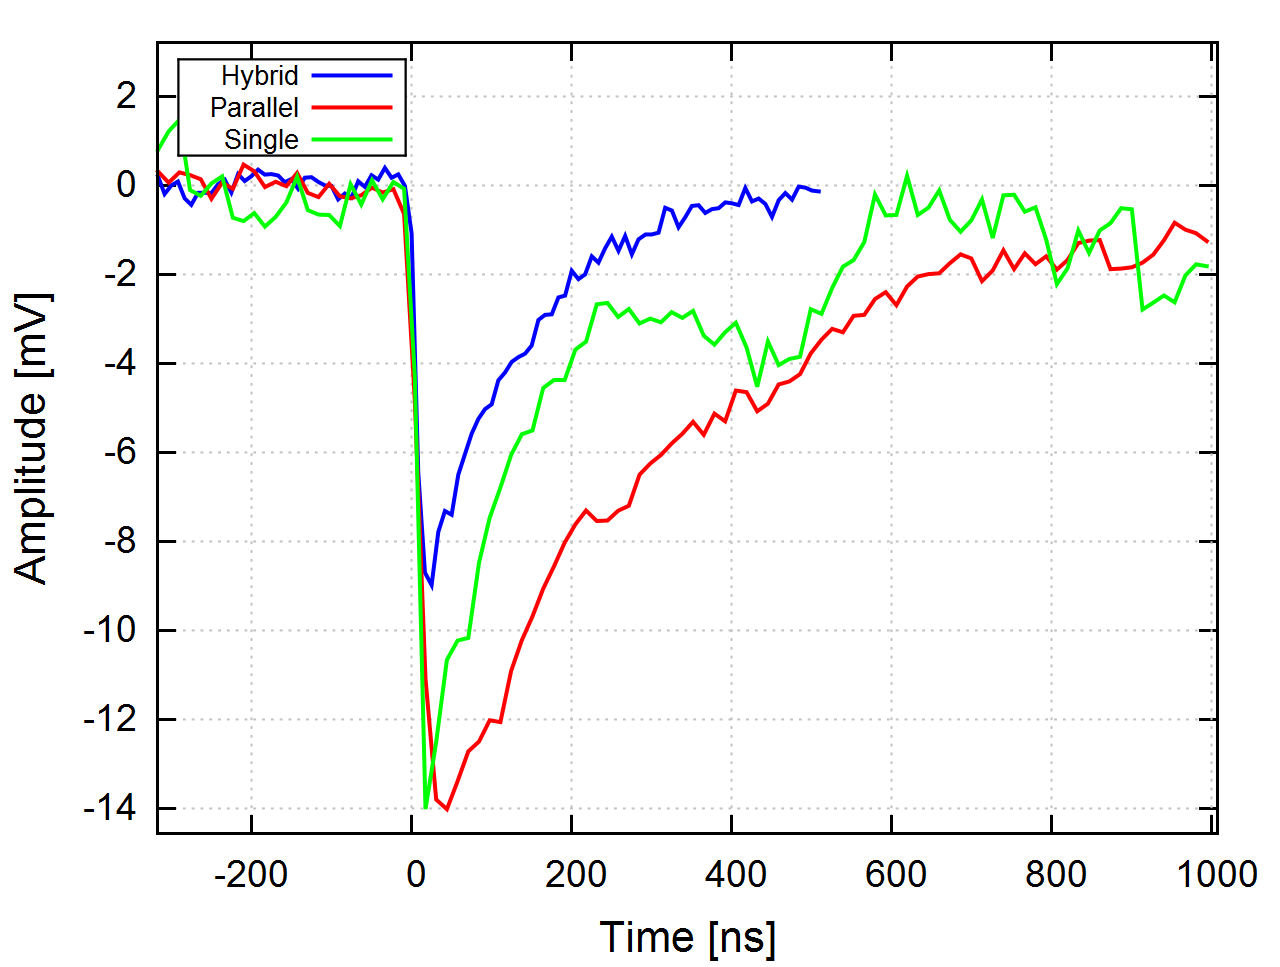
\includegraphics[width=0.24\textwidth]{./plots/signal/raw.png}}
	\hfill
	\subfloat[Amplified and normalized signal of blue (4x1 hybrid), red (4x1 parallel), green (1x1 single) with utilized photonique preamplifier] {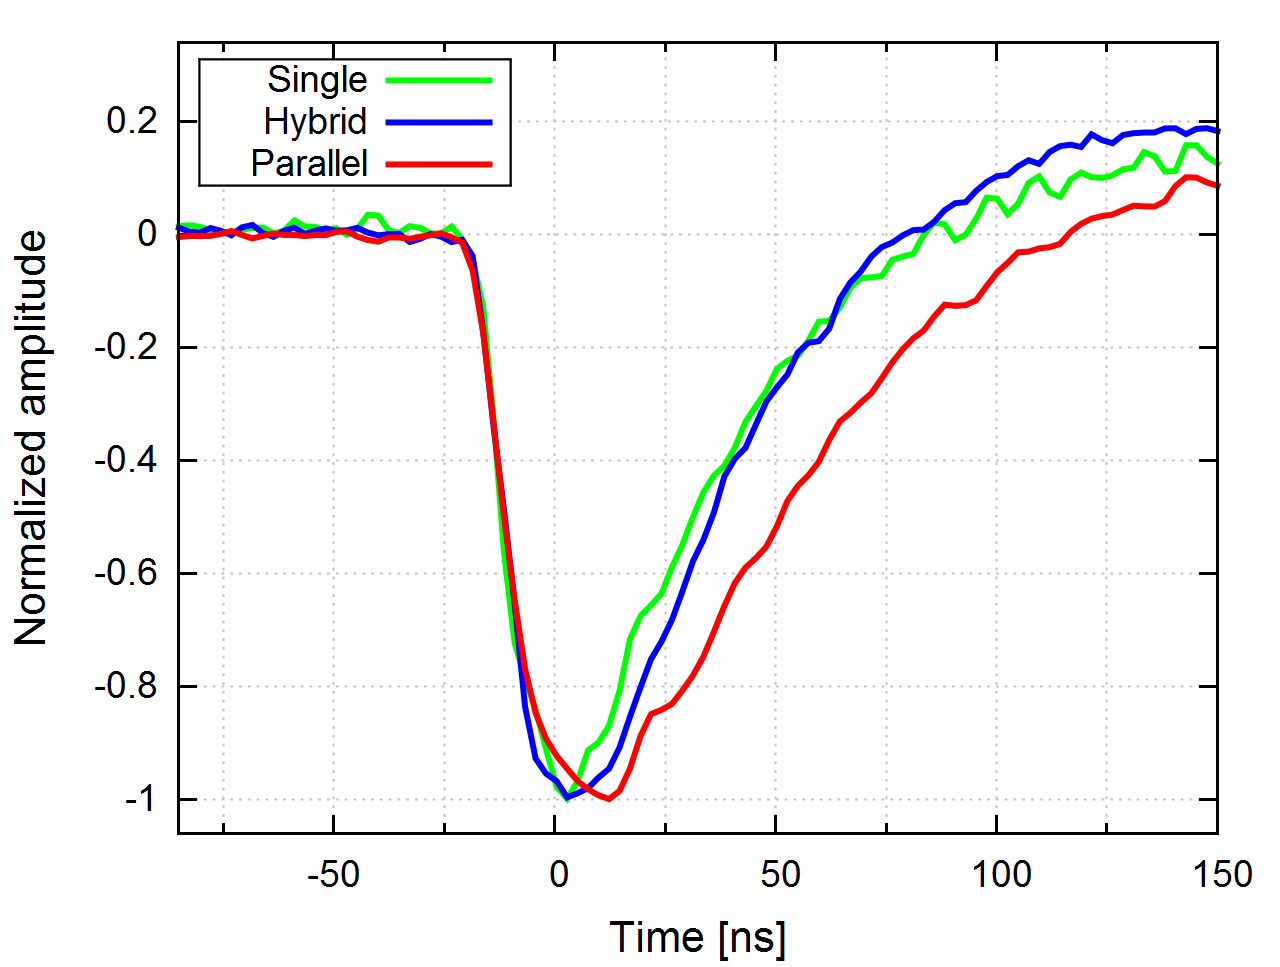
\includegraphics[width=0.24\textwidth]{./plots/signal/amp.png}}
	\hfill
	\caption{Raw and amplified signals of different SiPM configurations.}
	\label{fig:signals}
\end{figure}
As mentioned above, the signal strength depends on the number of SiPMs per board and on the configuration. The amplitude for the hybrid configuration gets divided by the square root of number of SiPMs utilized in the circuit where the parallel configuration has the same strength as a single SiPM. When using a preamplifier and normalizing the spectra one can see that the rise time of the hybrid board is fastest and the parallel board is slowest. Again, this suggests the use of hybrid boards for timing. \\ \indent
In preparation for the timing measurement the efficiency in counting and symmetry was tested. For this, two hybrid boards were mounted on each side on the scintillator and were connected via preamplifier to a leading edge discriminator. The output of those two channels were fed into a counter which was controlled by an external clock. A third channel was used to count the coincident counts of channel one and two. The threshold of the leading edge discriminator was set for both channels to satisfy the expected rate of cosmic muons in the scintillator. A \sr source with a small collimator was placed on several areas on top of the scintillator to create photoelectrons. \\
HEATMAP OF COUNTRATE \\
EXPLANATION OF ASYMMETRY \\
TIMING MEASUREMENT \\
ENERGY MEASUREMENT \\
RESUME 
     


%This sample document demonstrates proper use of REV\TeX~4.1 (and
%\LaTeXe) in mansucripts prepared for submission to APS
%journals. Further information can be found in the REV\TeX~4.1
%documentation included in the distribution or available at
%\url{http://authors.aps.org/revtex4/}.

%When commands are referred to in this example file, they are always
%shown with their required arguments, using normal \TeX{} format. In
%this format, \verb+#1+, \verb+#2+, etc. stand for required
%author-supplied arguments to commands. For example, in
%\verb+\section{#1}+ the \verb+#1+ stands for the title text of the
%author's section heading, and in \verb+\title{#1}+ the \verb+#1+
%stands for the title text of the paper.

%Line breaks in section headings at all levels can be introduced using
%\textbackslash\textbackslash. A blank input line tells \TeX\ that the
%paragraph has ended. Note that top-level section headings are
%automatically uppercased. If a specific letter or word should appear in
%lowercase instead, you must escape it using \verb+\lowercase{#1}+ as
%in the word ``via'' above.

%\subsection{\label{sec:level2}Second-level heading: %Formatting}

%This file may be formatted in either the %\texttt{preprint} or
%\texttt{reprint} style. \texttt{reprint} format %mimics final journal output. 
%Either format may be used for submission purposes. %\texttt{letter} sized paper should
%be used when submitting to APS journals.

%\subsubsection{Wide text (A level-3 head)}
%The \texttt{widetext} environment will make the text the width of the
%full page, as on page~\pageref{eq:wideeq}. (Note the use the
%\verb+\pageref{#1}+ command to refer to the page %number.) 
%\paragraph{Note (Fourth-level head is run in)}
%The width-changing commands only take effect in two-column formatting. 
%There is no effect if text is in a single column.

%\subsection{\label{sec:citeref}Citations and References}
%A citation in text uses the command \verb+\cite{#1}+ or
%\verb+\onlinecite{#1}+ and refers to an entry in the bibliography. 
%An entry in the bibliography is a reference to another document.

%\subsubsection{Citations}
%Because REV\TeX\ uses the \verb+natbib+ package of Patrick Daly, 
%the entire repertoire of commands in that package are available for your document;
%see the \verb+natbib+ documentation for further details. Please note that
%REV\TeX\ requires version 8.31a or later of \verb+natbib+.

%\paragraph{Syntax}
%The argument of \verb+\cite+ may be a single \emph{key}, 
%or may consist of a comma-separated list of keys.
%The citation \emph{key} may contain 
%letters, numbers, the dash (-) character, or the period (.) character. 
%New with natbib 8.3 is an extension to the syntax that allows for 
%a star (*) form and two optional arguments on the citation key itself.
%The syntax of the \verb+\cite+ command is thus (informally stated)
%\begin{quotation}\flushleft\leftskip1em
%\verb+\cite+ \verb+{+ \emph{key} \verb+}+, or\\
%\verb+\cite+ \verb+{+ \emph{optarg+key} \verb+}+, or\\
%\verb+\cite+ \verb+{+ \emph{optarg+key} \verb+,+ %\emph{optarg+key}\ldots \verb+}+,
%\end{quotation}\noindent
%where \emph{optarg+key} signifies 
%\begin{quotation}\flushleft\leftskip1em
%\emph{key}, or\\
%\texttt{*}\emph{key}, or\\
%\texttt{[}\emph{pre}\texttt{]}\emph{key}, or\\
%\texttt{[}\emph{pre}\texttt{]}\texttt{[}\emph{post}\texttt{]}\emph{key}, or even\\
%\texttt{*}\texttt{[}\emph{pre}\texttt{]}\texttt{[}\emph{post}\texttt{]}\emph{key}.
%\end{quotation}\noindent
%where \emph{pre} and \emph{post} is whatever text you %wish to place 
%at the beginning and end, respectively, of the %bibliographic reference
%Ref.~[\onlinecite{feyn54}]).
%(Keep in mind that no automatic space or punctuation is applied.)
%It is highly recommended that you put the entire \emph{pre} or \emph{post} portion 
%within its own set of braces, for example: 
%\verb+\cite+ \verb+{+ \texttt{[} %\verb+{+\emph{text}\verb+}+\texttt{]}\emph{key}\verb+}+.
%The extra set of braces will keep \LaTeX\ out of trouble if your \emph{text} contains the comma (,) character.

%The star (*) modifier to the \emph{key} signifies that the reference is to be 
%merged with the previous reference into a single bibliographic entry, 
%a common idiom in APS and AIP articles (see below, Ref.~[\onlinecite{epr}]). 
%When references are merged in this way, they are separated by a semicolon instead of 
%the period (full stop) that would otherwise appear.

%\paragraph{Eliding repeated information}
%When a reference is merged, some of its fields may be elided: for example, 
%when the author matches that of the previous reference, it is omitted. 
%If both author and journal match, both are omitted.
%If the journal matches, but the author does not, the journal is replaced by \emph{ibid.},
%as exemplified by Ref.~[\onlinecite{epr}]. 
%These rules embody common editorial practice in APS %and AIP journals and will only
%be in effect if the markup features of the APS and AIP %Bib\TeX\ styles is employed.
%\paragraph{The options of the cite command itself}
%Please note that optional arguments to the \emph{key} %change the reference in the bibliography, 
%not the citation in the body of the document. 
%For the latter, use the optional arguments of the %\verb+\cite+ command itself:
%\verb+\cite+ \texttt{*}\allowbreak
%\texttt{[}\emph{pre-cite}\texttt{]}\allowbreak
%\texttt{[}\emph{post-cite}\texttt{]}\allowbreak
%\verb+{+\emph{key-list}\verb+}+.

\bibliography{./bib}

\end{document}
%
% ****** End of file apssamp.tex ******
